\section{Tile-based Editor Calculus}\label{sec:formalism-2}

We now precisely characterize tile-based editing
as a calculus called \ty.
The punchline of \ty~ is the action judgment
$\performAction{\editState_1}{\action}{\editState_2}$,
which sends edit state $\editState_1$ to $\editState_2$
via action $\action$, and its governing invariant
that actions preserve parsability into a well-formed
program term.

We will begin our presentation in Section \ref{sec:zippers}
by describing the syntax of edit states $Z$.
Then, in Section \ref{sec:actions}, we will present each rule
defining the action judgment
$\performAction{\editState_1}{\action}{\editState_2}$,
describing supporting judgments and relevant metatheory
along the way.

\subsection{Zippers} \label{sec:zippers}

\begin{figure}
  \[\arraycolsep=3pt\begin{array}{rlrl}
      \text{zipper} & \zip & ::= & \zipper{\subject}{\zframe} \\
      \text{subject} & \subject & ::= &
        \pointing{\selection}{\selection} ~\vert~
        \selecting{\selection}{\selection}{\selection} ~\vert~
        \restructuring{\selection}{\selection}{\selection} \\
      \text{frame} & \zframe & ::= &
        \tfrelem^{\pat} ~\vert~ \tfrelem^{\expr}
 \end{array}\]
  \caption{
    Zipper syntax
  }
  \label{fig:zipper-syntax}
\end{figure}


Figure \ref{fig:zipper-syntax} shows the syntax of \ty~ edit states $\zip$,
which follow a variant of the well-known
\emph{zipper} pattern \cite{zipper}.
In particular, they have a \emph{bottom-up} zipper
structure---decomposing the total edit state $\zip$ into a
focused substructure $\subject$ and its surrounding context
$\zframe$---unlike the top-down structure used in other
work \cite{Hazelnut}.
In this work, we refer to $B$ as the \emph{subject} and $M$
as the \emph{frame}.

\paragraph{Subjects}
Subjects $\subject$ are modal, the three
variants corresponding to the pointing, selecting,
and restructuring modes we described using \tylr~
in Section \ref{sec:overview}.
Each mode decomposes the total subject into two
or three \emph{segments} $\selection$.
This decomposition encodes text-like cursor
placement between syntactic entities.
For example, consider the \tylr~ edit state
in pointing mode shown in Figure \ref{fig:pointing-zipper-example};
the corresponding subject in \ty~ is
$\pointing{\optile{\snumlit{1}}\bintile{\tprod}}{\optile{\snumlit{2}}}$.

\begin{figure}
\centering
\begin{subfigure}[c]{0.65\columnwidth}
  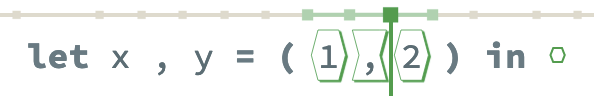
\includegraphics[width=\textwidth]{img/zipper-example-1.png}
  \caption{}\label{fig:pointing-zipper-example}
\end{subfigure}
\begin{subfigure}[c]{0.65\columnwidth}
  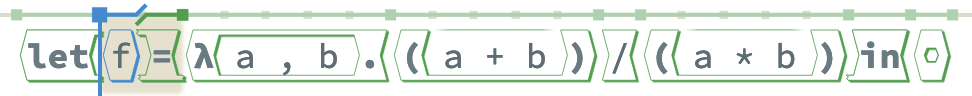
\includegraphics[width=\textwidth]{img/zipper-example-2.png}
  \caption{}\label{fig:selecting-zipper-example}
\end{subfigure}
\caption{\note{todo}}
\label{fig:zipper-examples}
\end{figure}

\begin{figure}
\[\arraycolsep=3pt\begin{array}{rlrl}
  \text{segment} & \selection & ::= &
  \selem_1\dots\selem_n \\
  \text{piece} & \selem & ::= &
    \tile ~\vert~
    \shard \\

  \text{tile} & \tile & ::= &
      \tile^{\pat} ~\vert~
      \tile^{\expr} \\

  \text{shard} & \shard & ::= &
    \shard^{\pat} ~\vert~
    \shard^{\expr}
\end{array}\]
\caption{
  Syntax of segments
}
\label{fig:segment-syntax}
\end{figure}
\begin{figure}
  \[\arraycolsep=4pt\begin{array}{rlrl}
    \text{pattern shard} & \shard^{\pat} & ::= &
      \shardlit{\texttt{(}} ~\vert~
      \shardlit{\texttt{)}} \\
    \text{expression shard} & \shard^{\expr} & ::= &
      \shardlit{\texttt{(}} ~\vert~
      \shardlit{\texttt{)}} ~\vert~
      \shardlit{$\lambda$} ~\vert~
      \shardlit{\texttt{.}} ~\vert~
      \shardlit{\texttt{let}} ~\vert~
      \shardlit{\texttt{=}} ~\vert~
      \shardlit{\texttt{in}}
  \end{array}\]
  \caption{Syntax of pattern and expression shards}
  \label{fig:shard-syntax-2}
\end{figure}


Segments $\selection$ are sequences of \emph{tiles}
and \emph{shards}, collectively called \emph{pieces},
as shown in Figure \ref{fig:segment-syntax}.
The two segments $\optile{\snumlit{1}}\bintile{\tprod}$ and
$\optile{\snumlit{2}}$ in the example above consist
entirely of expression tiles $\tile^{\expr}$,
the syntax for which was given in Figure \ref{fig:tile-syntax}.
Meanwhile, the subject of the \tylr~ edit state shown in
Figure \ref{fig:selecting-zipper-example}
% \begin{figure}[h]
%   \centering
%   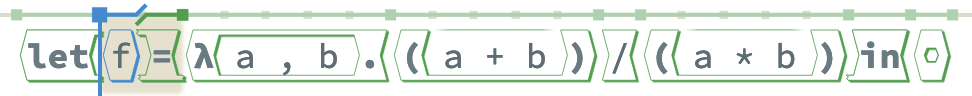
\includegraphics[width=0.65\columnwidth]{img/zipper-example-2.png}
% \end{figure}
is represented in \ty~ as
$\selecting{\shardlit{(}\optile{\snumlit{1}}\bintile{\tprod}}{\optile{\snumlit{2}}\shardlit{)}}{\cdot}$.
In this case, the first two segments $\shardlit{(}\optile{\snumlit{1}}\bintile{\tprod}$
and $\optile{\snumlit{2}}\shardlit{)}$
% (the third segment is the empty segment $\cdot$)
contain expression shards $\shard^{\expr}$,
the syntax for which is given in Figure \ref{fig:shard-syntax-2}.

\begin{figure}
  \vspace{-3px}
  \[
  \arraycolsep=3pt\begin{array}{rlrl}
      \mathsf{TilesFrame} & \tframe^s & ::= & \tframelit{\tiles^s\_\tiles^s}{\tfrelem^s} \\
      % \mathsf{Tile}^{\typ} & \tile^{\typ} & ::= &
      %     % \tnum ~\vert~
      %     \shole ~\vert~
      %     \sbool ~\vert~
      %     \snum ~\vert~
      %     \sarr{}{} ~\vert~
      %     \sprod{}{} ~\vert~
      %     \sparen{\tiles^{\typ}}\\
      \mathsf{PatTileFrame} & \tfrelem^{\pat} & ::= &
        \tframelit{\sparen{\_}}{\tframe^{\pat}} \\
      & & \vert &
        \tframelit{\slam{\_}{}}{\tframe^{\expr}} \\
      & & \vert &
        \tframelit{\slet{\_}{\tiles^{\expr}}{}}{\tframe^{\expr}} \\
      \mathsf{ExpTileFrame} & \tfrelem^{\expr} & ::= &
        \tframelit{\sparen{\_}}{\tframe^{\expr}} \\
      & & \vert &
        \tframelit{\slet{\tiles^{\pat}}{\_}{}}{\tframe^{\expr}}
        % \scond{}{\tiles^{\expr}}{}
  \end{array}\]
  \caption{
    Syntax of pattern and expression frames.
  }
  \label{fig:tile-syntax}
\end{figure}


\paragraph{Frames}
Frames model the rest of the edit state not included
in the subject.
At a high level, frames may be understood as a
list of nested containers,
arranged bottom-up such that the first container immediately
wraps the subject, each container other than the last points to its
parent container, and the last represents the edit state root.

The syntax for frames is given in Figure \ref{fig:frame-syntax}.
At the top level, frames $\zframe$ are sort-indexed \emph{tile frames}
$\tfrelem^s$, which represent tiles with a missing child of
sort $s$.
Other than the program root $\froot$, we annotate tile frame literals
with $\framehole$ symbols in place of the missing children.
Each tile frame $\tfrelem^s$ points to its parent
\emph{sequence frame} $\tframe^{s'}$, which carries the tile frame's
sibling tiles of sort $s'$.
Each sequence frame $\tframe^s$ in turn points to its parent
tile frame $\tfrelem^s$.
For example, the frames of the \tylr~ edit states in
Figure \ref{fig:zipper-examples} are represented in \ty~
as, respectively,
\[
  \tframelit{\sparen{\framehole}}{
    \tframelit{\cdot\framehole\cdot}{
      \tframelit{\tlet{\sprod{\svar{x}}{\svar{y}}}{\framehole}}{
        \tframelit{\cdot\framehole\optile{\ophole}}{\froot}
      }
    }
  }
\]
and
\[
  \tframelit{\tlet{\sprod{\svar{x}}{\svar{y}}}{\framehole}}{
    \tframelit{\cdot\framehole\optile{\ophole}}{\froot}
  }.
\]

\subsection{Actions} \label{sec:actions}

\begin{figure}
  \vspace{-3px}
  \[
  \arraycolsep=3pt\begin{array}{rlrl}
      \mathsf{Action} & \action & ::= &
        \actionlit{mark} ~\vert~
        \actionlit{move}~\direction ~\vert~
        \actionlit{delete} ~\vert~
        \actionlit{construct}~\tile^s \\
      \mathsf{Direction} & \direction & ::= &
        \texttt{left} ~\vert~
        \texttt{right}
  \end{array}\]
  \caption{Syntax of actions}
  \label{fig:action-syntax}
\end{figure}


Figure \ref{fig:action-syntax} gives the syntax of actions $\action$.
We will now describe each of the eight rules defining the
action judgment $\performAction{\editState_1}{\action}{\editState_2}$.

In these rules, we aim to support a one-dimensional interaction
model, where the client may view the total edit
state as its serialization, navigate through it
in a linear fashion, and select arbitrary subranges.
Toward these ends, actions in \ty~ rely
on a form of incremental unparsing and reparsing by which
hierarchical structures may be temporarily ``flattened'' as needed,
as we will first encounter in the next section.

% \note{introduce action syntax}

% \note{remark on first two rules taking the longest to establish setup,
% after which remaining six rules build on top of that}

% Our design of zipper operations diverges from prior art
% in our pursuit of linear text-like interactivity.
% Prior zipper designs are strictly hierarchical and ask
% the client to navigate in a structure-aware two-dimensional
% fashion: left and right to traverse siblings,
% up and down to traverse parent-child relations.
% In contrast, we aim to support a one-dimensional interaction
% model:
% it should be possible to navigate freely by moving solely
% left and right \note{might need to clarify or change wording
% here to address comparison with ordered traversals of trees};
% furthermore it should be possible to specify
% arbitrary subranges of a one-dimensional serialization
% of the total structure.
% Toward these ends, actions in \ty~ rely
% on a form of incremental unparsing and reparsing by which
% hierarchical structures may be ``flattened'' as needed
% to support linear traversal and partial selection.


\subsubsection{Moving}

We start with basic movement, the rule for which is shown below.
Movement in each mode defers to an internally recursive auxiliary
judgment, in this case $\pmove{\editState_1}{\direction}{\editState_2}$,
defined in Figure \ref{fig:move-pointing}.
\[
  \inferrule[Move]{
    \pmove{\zipper{\pointing{\selection_1}{\selection_2}}{\zframe}}{\direction}{\editState}
  }{
    \performAction{
      \zipper{\pointing{\selection_1}{\selection_2}}{\zframe}
    }{
      \actionlit{move}\ \direction
    }{
      \editState
    }
  }
\]

\begin{figure}
  \judgbox{\pmove{\editState_1}{\direction}{\editState_2}}{$\editState_1$ transitions via movement $\direction$ to $\editState_2$\\\ \ in pointing mode}
  \begin{mathpar}
  \inferrule[PMoveRightAtomic]{
    \disassemblesDown{\selem}{\cdot}
  }{
    \pmove{
      \zipper{\pointing{\selection_1}{\selem\selection_2}}{\zframe}
    }{
      \texttt{right}
    }{
      \parseZipper{\zipper{\pointing{\parseSelection{\selection_1\selem}}{\selection_2}}{\zframe}}
    }
  }

  \inferrule[PMoveRightDisassembles]{
    \disassemblesDown{\selem}{\selection_3} \\
    \selection_3\neq\cdot \\
    \pmove{
      \zipper{\pointing{\selection_1}{\selection_3\selection_2}}{\zframe}
    }{
      \texttt{right}
    }{
      \zip
    }
  }{
    \pmove{
      \zipper{\pointing{\selection_1}{\selem\selection_2}}{\zframe}
    }{
      \texttt{right}
    }{
      \zip
    }
  }

  \inferrule[PMoveRightFrame]{
    \disassemblesUp{
      \zframe
    }{
      \zipper{\pointing{\selection_2}{\selection_3}}{\zframe'}
    } \\
    \pmove{
      \zipper{\pointing{\selection_2\selection_1}{\selection_3}}{\zframe'}
    }{
      \texttt{right}
    }{
      \zip
    }
  }{
    \pmove{
      \zipper{\pointing{\selection_1}{\cdot}}{\zframe}
    }{
      \texttt{right}
    }{
      \zip
    }
  }
\end{mathpar}

\vspace{-2px}
\CaptionLabel{Movement in pointing mode}{fig:move-pointing}
\vspace{-2px}
\end{figure}


\note{---break---}

We can produce shards from tiles via \emph{step-disassembly},
as defined for pieces and segments in Figure \ref{fig:subject-disassembly}.
The first judgment $\pieceDisassembles{\selem}{\selection}$
step-disassembles a piece $\selem$ into a segment of
its constituent shards and children tiles.
The second judgment $\stepDisassembleSelection{\selection_1}{\selection_2}$
chooses a piece in $\selection_1$ and replaces it with its
step-disassemblage to produce $\selection_2$.
The reflexive transitive closure $\tpiecesdd^*$ of
$\tpiecesdd$ we call \emph{disassembly}.
\note{give examples from overview}

\begin{figure}
  \judgbox{\pieceDisassembles{\selem}{\selection}}{$\selem$ step-disassembles to $\selection$}
  \[
    \arraycolsep=3pt
    \begin{array}{rcl}
      \optile{\sparen{\tiles^s}} & \tpiecedd & \shardlit{\texttt{(}}~\tiles^s~\shardlit{\texttt{)}} \\
      \pretile{\tlam{\tiles^{\pat}}} & \tpiecedd & \shardlit{\lambda}~\tiles^{\pat}~\shardlit{\texttt{.}} \\
      \pretile{\tlet{\tiles^{\pat}}{\tiles^{\expr}}} & \tpiecedd & \shardlit{\texttt{let}}~\tiles^{\pat}~\shardlit{\texttt{=}}~\tiles^{\expr}~\shardlit{\texttt{in}} \\
      \text{otherwise\hspace{0.5cm}} \selem & \tpiecedd & \cdot
  \end{array}\]
  \vspace{0.1cm}

  \judgbox{\stepDisassembleSelection{\selection_1}{\selection_2}}{$\selection_1$ step-disassembles to $\selection_2$}
  \begin{mathpar}
    \inferrule[]{
      \pieceDisassembles{\selem}{\selection}
    }{
      \stepDisassembleSelection{\selem}{\selection}
    }\hspace{30pt}
    \inferrule[]{
      \stepDisassembleSelection{\selection_1}{\selection'_1}
    }{
      \stepDisassembleSelection{\selection_1\selection_2}{\selection'_1\selection_2}
    }\hspace{30pt}
    \inferrule[]{
      \stepDisassembleSelection{\selection_2}{\selection'_2}
    }{
      \stepDisassembleSelection{\selection_1\selection_2}{\selection_1\selection'_2}
    }
  \end{mathpar}
  \caption{
    Step-disassembly of pieces and segments
  }
  \label{fig:subject-disassembly}
\end{figure}

Disassembly of segments is analogous to string derivation for a
context-free grammar (CFG),
where a string containing terminal and nonterminal symbols is iteratively
rewritten according to the grammar rules.
A parser for a CFG may then be characterized as a function
that takes a string of terminal symbols and identifies,
if any exist,
a derivation from the grammar's starting nonterminal
symbol to the input string.
We may similarly characterize a parser on pieces according
to the disassembly relation.
In this case, however, our parsing goal is maximal,
not maximum, structure, \ie, the parser
need not identify a disassembly connecting the input
shards to unbroken tiles (the start symbol), but need only assemble shards
together opportunistically.
\note{too hand-wavey, come back and revise}

More precisely, we can show that disassembly is a
partial order, and that every segment in this order
has a unique maximal segment that disassembles to it.
\begin{lemma}
  $\tpiecesdd^*$ is a partial order.
\end{lemma}
\begin{lemma}\label{lemma:unique-parsed-selection}
  For every segment $\selection$, there exists a unique
  segment $\parseSelection{\selection}$ such that:
  \begin{itemize}
  \item $\parseSelection{\selection}\searrow^*\selection$, and
  \item $\parseSelection{\selection}$ is maximal: if $\selection'\searrow^*\parseSelection{\selection}$ then $\selection' = \parseSelection{\selection}$.
  \end{itemize}
\end{lemma}
\noindent
We say that the operator $\parseSelection{\cdot}$ performs \emph{segment assembly}.
We defer presenting a constructive implementation of segment
assembly to the yet-imaginary appendix.

\note{---break---}

Like tiles, frames may be decomposed into their
lexically constituent tiles and tokens via the
\emph{frame disassembly} function $\disassembleTileFrame{\cdot}$,
defined in Figure \note{ref}.
Similar to how we lift tile disassembly to selection
disassembly, we can lift frame disassembly to
\emph{edit state step-disassembly}, defined in Figure \note{ref}.
We can show that the reflexive transitive closure
$\nearrow^*$ of $\nearrow$, which we call \emph{edit state disassembly},
is a partial order in
which every edit state with a subject in pointing mode
has a unique minimal element that disassembles to it:
\begin{lemma}
  $\nearrow^*$ is a partial order.
\end{lemma}
\begin{lemma}\label{lemma:unique-parsed-editstate}
  For every zipper $\editState = \zipper{\pointing{\selection_1}{\selection_2}}{\tfrelem^s}$
  in pointing mode,
  there exists a unique zipper $\parseZipper{\editState}$ such that
  \begin{itemize}
  \item $\parseZipper{\editState} \nearrow^* \editState$, and
  \item $\parseZipper{\editState}$ is minimal: if $\editState' \nearrow^* \parseZipper{\editState}$ then $\editState' = \parseZipper{\editState}$.
  \end{itemize}
\end{lemma}
\noindent
We say that the operator $\parseZipper{\cdot}$ performs \emph{zipper assembly}.

\begin{figure}
  \vspace{-3px}
  \[
  \setlength{\fboxsep}{1pt}
  \arraycolsep=3pt\def\arraystretch{1.4}\begin{array}{rcl}
      \disassembleTileFrame{
        \tframelit{
          \sparen{\_}
        }{
          \tframelit{\tiles^s_1\_\tiles^s_2}{\tfrelem^{\pat}}
        }
      } & = &
        \zipper{
          \pointing{\tiles^s_1\tokenLit{\texttt{(}}~}{~\tokenLit{\texttt{)}}\tiles^s_2}
        }{
          \tfrelem^{\pat}
        } \\

      \disassembleTileFrame{
        \tframelit{
          \slam{\_}{}
        }{
          \tframelit{\tiles^{\expr}_1\_\tiles^{\expr}_2}{\tfrelem^{\expr}}
        }
      } & = &
        \zipper{
          \pointing{\tiles^{\expr}_1\tokenLit{\lambda}~}{~\tokenLit{\texttt{.}}\tiles^{\expr}_2}
        }{
          \tfrelem^{\expr}
        } \\

      \disassembleTileFrame{
        \tframelit{
          \slet{\_}{\tiles^{\expr}_0}{}
        }{
          \tframelit{\tiles^{\expr}_1\_\tiles^{\expr}_2}{\tfrelem^{\expr}}
        }
      } & = & \\
        \zipper{
          \pointing{
            \tiles^{\expr}_1\tokenLit{\texttt{let}}~
          }{
            ~\tokenLit{\texttt{=}}~\tiles^{\expr}_0\tokenLit{\texttt{in}}~\tiles^{\expr}_2
          }
        }{
          \tfrelem^{\expr}
        } \\

      \disassembleTileFrame{
        \tframelit{
          \slet{\tiles^{\pat}}{\_}{}
        }{
          \tframelit{\tiles^{\expr}_1\_\tiles^{\expr}_2}{\tfrelem^{\expr}}
        }
      } & = & \\
        \zipper{
          \pointing{
            \tiles^{\expr}_1\tokenLit{\texttt{let}}~\tiles^{\pat}~\tokenLit{\texttt{=}}~
          }{
            ~\tokenLit{\texttt{in}}~\tiles^{\expr}_2
          }
        }{
          \tfrelem^{\expr}
        }
  \end{array}\]
  \caption{
    Disassembling a tile frame.
  }
  \label{fig:disassemble-tile}
\end{figure}
\begin{figure}
  \judgbox{\disassembleZipper{\editState_1}{\editState_2}}{$\editState_1$ step-disassembles up to $\editState_2$}
  \begin{mathpar}
    \inferrule[]{
      \disassemblesUp{\zframe}{\zipper{\pointing{\selection_3}{\selection_4}}{\zframe'}}
    }{
      \disassembleZipper{
        \zipper{\pointing{\selection_1}{\selection_2}}{\zframe}
      }{
        \zipper{\pointing{\selection_3\selection_1}{\selection_2\selection_4}}{\zframe'}
      }
    }
  \end{mathpar}
  \caption{
    Step-disassembly of a zipper
  }
  \label{fig:disassemble-zipper}
  \end{figure}

\subsubsection{Constructing}
\[
  \inferrule[Construct]{
    \fixHolesSelections{\selection_1}{\tile^s\selection_2}{s}{\selection'_1}{\selection'_2}
  }{
    \performAction{
      \zipper{\pointing{\selection_1}{\selection_2}}{\tfrelem^s}
    }{
      \actionlit{construct}\ \tile^s
    }{
      \zipper{\pointing{\selection'_1}{\selection'_2}}{\tfrelem^{s}}
    }
  }
\]

We characterize assembly of pieces into terms
similarly to how we characterized segment assembly
in Section \ref{sec:shards-and-pieces}.
Figure \ref{fig:flatten-term} defines the \emph{term
disassembly} judgments $\flattenTerm{p}{\selection}$
and $\flattenTerm{e}{\selection}$, which decompose
the terms $p$ and $e$ into segments $\selection$.

\begin{figure}
  \judgbox{\flattenTerm{p}{\tiles^{\pat}}}{$p$ flattens to $\tiles^{\pat}$}
  \begin{mathpar}
    \inferrule[]{
    }{
      \flattenTerm{\term{\ophole}}{\optile{\ophole}}
    }\hspace{20pt}
    \inferrule[]{
    }{
      \flattenTerm{\term{\svar{x}}}{\optile{\svar{x}}}
    }\hspace{20pt}
    \inferrule[]{
      \flattenTerm{p}{\tiles^{\pat}}
    }{
      \flattenTerm{\term{\sparen{p}}}{\optile{\sparen{\tiles^{\pat}}}}
    }\\
    \inferrule[]{
      \flattenTerm{p_1}{\tiles^{\pat}_1} \\
      \flattenTerm{p_2}{\tiles^{\pat}_2}
    }{
      \flattenTerm{\term{\sbinhole{p_1}{p_2}}}{\tiles^{\pat}_1~\bintile{\binhole}~\tiles^{\pat}_2}
    }\hspace{20pt}
    \inferrule[]{
      \flattenTerm{p_1}{\tiles^{\pat}_1} \\
      \flattenTerm{p_2}{\tiles^{\pat}_2}
    }{
      \flattenTerm{\term{\sprod{p_1}{p_2}}}{\tiles^{\pat}_1~\bintile{\tprod}~\tiles^{\pat}_2}
    }
  \end{mathpar}

  \vspace{10pt}
  \judgbox{\flattenTerm{e}{\tiles^{\expr}}}{$e$ flattens to $\tiles^{\expr}$}
  \begin{mathpar}
    \inferrule[]{
    }{
      \flattenTerm{\term{\ophole}}{\optile{\ophole}}
    }\hspace{15pt}
    \inferrule[]{
    }{
      \flattenTerm{\term{\snumlit{n}}}{\optile{\snumlit{n}}}
    }\hspace{15pt}
    \inferrule[]{
    }{
      \flattenTerm{\term{\svar{x}}}{\optile{\svar{x}}}
    }\hspace{15pt}
    \inferrule[]{
      \flattenTerm{e}{\tiles^{\expr}}
    }{
      \flattenTerm{\term{\sparen{e}}}{\optile{\sparen{\tiles^{\expr}}}}
    }\\
    \inferrule[]{
      \flattenTerm{e_1}{\tiles^{\expr}_1} \\
      \flattenTerm{e_2}{\tiles^{\expr}_2}
    }{
      \flattenTerm{\term{\sbinhole{e_1}{e_2}}}{\tiles^{\expr}_1~\bintile{\binhole}~\tiles^{\expr}_2}
    }\hspace{20pt}
    \inferrule[]{
      \flattenTerm{e_1}{\tiles^{\expr}_1} \\
      \flattenTerm{e_2}{\tiles^{\expr}_2}
    }{
      \flattenTerm{\term{\sprod{e_1}{e_2}}}{\tiles^{\expr}_1~\bintile{\tprod}~\tiles^{\expr}_2}
    }\\
    \inferrule[]{
      \flattenTerm{p}{\tiles^{\pat}} \\
      \flattenTerm{e}{\tiles^{\expr}}
    }{
      \flattenTerm{\term{\slam{p}{e}}}{\pretile{\tlam{\tiles^{\pat}}}~\tiles^{\expr}}
    }\\
    \inferrule[]{
      \flattenTerm{p}{\tiles^{\pat}} \\
      \flattenTerm{e_1}{\tiles^{\expr}_1} \\
      \flattenTerm{e_2}{\tiles^{\expr}_2}
    }{
      \flattenTerm{\term{\slet{p}{e_1}{e_2}}}{\pretile{\tlet{\tiles^{\pat}}{\tiles^{\expr}_1}}~\tiles^{\expr}_2}
    }
  \end{mathpar}

  \caption{
    Term flattening
  }
  \label{fig:flatten-term}
  \end{figure}

The segments produced by term disassembly always satisfy
a couple properties. First, they are always \emph{intact}:
\begin{definition}
  A segment $\selection$ is called \emph{intact} if it consists
  solely of tiles.
\end{definition}
\begin{lemma}
  If $\flattenTerm{p}{\selection}$ or $\flattenTerm{e}{\selection}$ then $\selection$ is intact.
\end{lemma}
\note{call back to initial \tylr~ figure showing term
vs tile view of lambda term}

Second, each piece in a term disassemblage ``fits''
its neighbors, \ie, each piece's left and right \emph{tips}
match, respectively, the right tip of its left neighbor
and the left tip of its right neighbor.
We have suggestively notated the tile and shard forms with
approximations of their tips, but have elided some relevant
sort information.
More completely, we define in Figure \ref{fig:piece-tips}
the syntax for tips and the operators $\leftTip{c}$
and $\rightTip{c}$ that return the left and right tips
of a piece $c$.
\note{describe tips, discuss a tile example and
a shard example}

In fact, this notion of ``fit'' extends to all disassemblages
of a disassembled term. \note{todo: different names for term
disassembly vs tile disassembly}
More precisely, Figure \ref{fig:tip-tip-connected} defines
\emph{$\tau_1\tau_2$-connectedness} of a segment.
\note{a little more discussion, example of connected vs not connected segment}
We say that a segment $\selection$ is \emph{connected} if there exist
tips $\tau_1$ and $\tau_2$ such that $\selection$ is $\tau_1\tau_2$-connected.

\begin{lemma}
  If $\flattenTerm{p}{C}$ then $C$ is $\lltip{\pat}~\rrtip{\pat}$-connected.
  If $\flattenTerm{e}{C}$ then $C$ is $\lltip{\expr}~\rrtip{\expr}$-connected.
  \note{todo: sort-indexed terms}
\end{lemma}

\begin{figure}
  \[\arraycolsep=3pt\begin{array}{rlrl}
    \text{tip} & \tip & ::= & \lltip{s} ~\vert~ \rrtip{s}
  \end{array}\]

  \begin{minipage}[t]{0.6\columnwidth}\vspace{0pt}
    \begin{tabular}{|l|ll|}
      $\tile$ & \strut$\leftTip{\tile}$ & $\rightTip{\tile}$ \\
      \hline
      $\optile{\ophole}^{s}$ & $\lltip{s}$ & $\rrtip{s}$ \\
      $\optile{\svar{x}}^s$ & $\lltip{s}$ & $\rrtip{s}$ \\
      $\optile{\snumlit{n}}$ & $\lltip{\expr}$ & $\rrtip{\expr}$ \\
      $\optile{\sparen{\_}}^s$ & $\lltip{s}$ & $\rrtip{s}$ \\
      $\bintile{\binhole}^s$ & $\rrtip{s}$ & $\lltip{s}$ \\
      $\bintile{\tprod}^s$ & $\rrtip{s}$ & $\lltip{s}$ \\
      $\pretile{\tlam{\_}}$ & $\lltip{\expr}$ & $\lltip{\expr}$ \\
      $\pretile{\tlet{\_}{\_}}$ & $\lltip{\expr}$ & $\lltip{\expr}$
    \end{tabular}
    \end{minipage}
    \begin{minipage}[t]{0.35\columnwidth}\vspace{0pt}
    \begin{tabular}{|l|ll|}
      $\shard$ & \strut$\leftTip{\shard}$ & $\rightTip{\shard}$ \\
      \hline
      $\shardlit{(}^s$ & $\lltip{s}$ & $\lltip{s}$ \\
      $\shardlit{)}^s$ & $\rrtip{s}$ & $\rrtip{s}$ \\
      $\shardlit{$\lambda$}$ & $\lltip{\expr}$ & $\lltip{\pat}$ \\
      $\shardlit{.}$ & $\rrtip{\pat}$ & $\lltip{\expr}$ \\
      $\shardlit{let}$ & $\lltip{\expr}$ & $\lltip{\pat}$ \\
      $\shardlit{=}$ & $\rrtip{\pat}$ & $\lltip{\expr}$ \\
      $\shardlit{in}$ & $\rrtip{\expr}$ & $\lltip{\expr}$
    \end{tabular}
    \end{minipage}
  \caption{The syntax of tips. Left and right tips of pieces. \note{wtf latex why won't you align}}
  \label{fig:piece-tips}
\end{figure}
\begin{figure}
  \judgbox{
    \text{$\selection$ is $\tau_1\tau_2$-connected}
  }{}
  \begin{mathpar}
    \inferrule[]{
      \nsegmentdd{\selem} \\
      \leftTip{\selem} = \tau_1 \\
      \rightTip{\selem} = \tau_2
    }{
      \text{$\selem$ is $\tau_1\tau_2$-connected}
    }

    \inferrule[]{
      \pieceDisassembles{\selem}{\selection} \\
      \text{$\selection$ is $\tau_1\tau_2$-connected}
    }{
      \text{$\selem$ is $\tau_1\tau_2$-connected}
    }

    \inferrule[]{
      \text{$\selection_1$ is $\tau_1\tau_2$-connected} \\
      \text{$\selection_2$ is $\tau_2\tau_3$-connected}
    }{
      \text{$\selection_1\selection_2$ is $\tau_1\tau_3$-connected}
    }
  \end{mathpar}

  \caption{Connected segments}
  \label{fig:tip-tip-connected}
\end{figure}


These two properties of segments---intactness
and connectedness---are in fact also \emph{sufficient} to
guarantee there exists a term that disassembles to
the segment in question.

\begin{theorem} \label{thm:term-parseability}
  A segment $\selection$ is intact and $\lltip{s}~\rrtip{s}$-connected
  if and only if there exists a term $x$ of sort $s$ such that
  $\flattenTerm{x}{\selection}$.
  \note{todo: sort-indexed terms}
\end{theorem}
\noindent
We call such a segment an \emph{opseq of sort $s$}.
\note{move above theorem, state theorem in terms of that}

\paragraph{Hole fixing}
We have seen in Section \ref{sec:overview} how tile-based
editing supports temporary departure from intactness of
the edit state while selecting and restructuring.
However, edit actions must take care to maintain
connectedness at all times to preserve opseq structure
upon reassembling shards and returning to pointing mode.

\begin{figure}
  \judgbox{
    \fixHolesSelection{\rTip_1}{\selection_1}{\selection_2}{\rTip_2}
  }{
    $\selection_1$ is hole fixed under tip constraint $\rTip_1$ \\
    to produce $\selection_2$ and new tip constraint $\rTip_2$
  }
  \begin{mathpar}
    \inferrule[]{
    }{
      \fixHolesSelection{r}{\cdot}{\cdot}{r}
    } \\
    \inferrule[]{
      \text{\note{$\psi$ is a hole}} \\
      \fixHolesSelection{r}{\selection}{\selection'}{r'}
    }{
      \fixHolesSelection{r}{\selem\selection}{\selection'}{r'}
    } \\
    \inferrule[]{
      \text{\note{$\psi$ not a hole}} \\
      \fits{r}{\leftTip{\selem}} \\
      \fixHolesSelection{\rightTip{\selem}}{\selection}{\selection'}{r'}
    }{
      \fixHolesSelection{r}{\selem\selection}{\selection'}{r'}
    } \\
    \inferrule[]{
      \text{\note{$\psi$ not a hole}} \\
      \leftTip{\selem} = \ltipconc{s} \\
      \fixHolesSelection{\rightTip{\selem}}{\selection}{\selection'}{r'}
    }{
      \fixHolesSelection{\rtipconc{s}}{\selem\selection}{\ophole^s\selem\selection'}{r'}
    } \\
    \inferrule[]{
      \text{\note{$\psi$ not a hole}} \\
      \leftTip{\selem} = \ltipconv{s} \\
      \fixHolesSelection{\rightTip{\selem}}{\selection}{\selection'}{r'}
    }{
      \fixHolesSelection{\rtipconv{s}}{\selem\selection}{\binhole^s\selem\selection'}{r'}
    } \\
  \end{mathpar}

  \judgbox{
    \fixHolesSelections{\rTip}{\selection_1}{\selection_2}{\lTip}{\selection_3}{\selection_4}
  }{$\selection_1$ and $\selection_2$ are hole fixed under \\
    tip constraints $\rTip$ and $\lTip$ \\
    to produce $\selection_3$ and $\selection_4$
  }
  \vspace{10pt}
  \begin{mathpar}
    \inferrule[]{
      \fixHolesSelection{r}{\selection_1}{\selection'_1}{r'} \\
      \fixHolesSelection{r'}{\selection_2}{\selection'_2}{r''} \\
      \fits{r''}{l}
    }{
      \fixHolesSelections{r}{\selection_1}{\selection_2}{l}{\selection'_1}{\selection'_2}
    } \\
    \inferrule[]{
      \fixHolesSelection{r}{\selection_1}{\selection'_1}{r'} \\
      \fixHolesSelection{r'}{\selection_2}{\selection'_2}{\rtipconc{s}}
    }{
      \fixHolesSelections{r}{\selection_1}{\selection_2}{\ltipconc{s}}{\selection'_1}{\selection'_2\ophole^s}
    }
  \end{mathpar}
  \caption{
    Hole fixing
  }
  \label{fig:fixholes-2}
  \end{figure}

Toward this end, we will see that actions make use of the hole fixing judgment
$\fixHolesSelections{\selection_1}{\selection_2}{s}{\selection'_1}{\selection'_2}$
given in Figure \ref{fig:fixholes-2},
which takes a pair of segments $\selection_1$ and $\selection_2$
and inserts and removes holes of sort $s$ to produce $\selection'_1$
and $\selection'_2$.
\note{add discussion of auxiliary judgment}
Hole fixing is governed by the following lemma.

\note{need to explain how I'm dropping holes along the way.}
\note{examples for the two rules where holes are inserted in auxiliary judgment.}

\begin{lemma}
  Suppose $\selection_1$ and $\selection_2$ are connected segments
  and $\fixHolesSelections{\selection_1}{\selection_2}{s}{\selection'_1}{\selection'_2}$.
  Then,
  \begin{enumerate}
    \item $\selection'_1\selection'_2$ is $\lltip{s}\rrtip{s}$-connected;
    \item $\selection'_1$ and $\selection'_2$ consist of the same non-hole pieces as
        $\selection_1$ and $\selection_2$ respectively; and
    \item there exist no neighboring holes in $\selection'_1\selection'_2$.
  \end{enumerate}
  \note{formalize 2 (note same order) and 3}
\end{lemma}


\subsubsection{Selecting}
\[
  \inferrule[StartSelecting]{
  }{
    \performAction{
      \zipper{\pointing{\selection_1}{\selection_2}}{\zframe}
    }{
      \actionlit{mark}
    }{
      \zipper{\selecting{\selection_1}{\strut~\cdot~}{\selection_2}}{\zframe}
    }
  }
\]

\[
  \inferrule[Select]{
    \smove{\zipper{\selecting{\selection_1}{\selection_2}{\selection_3}}{\zframe}}{\direction}{\editState}
  }{
    \performAction{
      \zipper{\selecting{\selection_1}{\selection_2}{\selection_3}}{\zframe}
    }{
      \actionlit{move}\ \direction
    }{
      \editState
    }
  }
\]

\begin{figure}
  \judgbox{\smove{\editState_1}{\direction}{\editState_2}}{$\editState_1$ moves to $\editState_2$ in selecting mode}
  \begin{mathpar}

\inferrule[SMoveLeftAtomic]{
  \nsegmentdd{\selem} \\
  \parseSelection{\selem\selection_2} = \selection'_2
}{
  \smove{
    \zipper{\selecting{\selection_1\selem}{\selection_2}{\selection_3}}{\zframe}
  }{
    \texttt{left}
  }{
    \zipper{\selecting{\selection_1}{\selection'_2}{\selection_3}}{\zframe}
  }
}

\inferrule[SMoveLeftDisassembles]{
  \pieceDisassembles{\selem}{\selection_4} \\
  \smove{
    \zipper{\selecting{\selection_1\selection_4}{\selection_2}{\selection_3}}{\zframe}
  }{
    \texttt{left}
  }{
    \zip
  }
}{
  \smove{
    \zipper{\selecting{\selection_1\selem}{\selection_2}{\selection_3}}{\zframe}
  }{
    \texttt{left}
  }{
    \zip
  }
}

\inferrule[SMoveLeftFrame]{
  \framedu{
    \zframe
  }{
    \zipper{\pointing{\selection_3}{\selection_4}}{\zframe'}
  } \\
  \smove{
    \zipper{\selecting{\selection_3}{\selection_1}{\selection_2\selection_4}}{\zframe'}
  }{
    \texttt{left}
  }{
    \zip
  }
}{
  \smove{
    \zipper{\selecting{\cdot}{\selection_1}{\selection_2}}{\zframe}
  }{
    \texttt{left}
  }{
    \zip
  }
} \\

\inferrule[SMoveRightAtomic]{
  \nsegmentdd{\selem} \\
  \parseZipper{\zipper{\pointing{\parseSelection{\selection_1\selem}}{\selection_3}}{\zframe}} =
    \zipper{\pointing{\selection'_1}{\selection'_3}}{\zframe'}
}{
  \smove{
    \zipper{\selecting{\selection_1}{\selem\selection_2}{\selection_3}}{\zframe}
  }{
    \texttt{right}
  }{
    \zipper{\selecting{\selection'_1}{\selection_2}{\selection'_3}}{\zframe'}
  }
}

\inferrule[SMoveRightDisassembles]{
  \pieceDisassembles{\selem}{\selection_4} \\
  \smove{
    \zipper{\selecting{\selection_1}{\selection_4\selection_2}{\selection_3}}{\zframe}
  }{
    \texttt{right}
  }{
    \zip
  }
}{
  \smove{
    \zipper{\selecting{\selection_1}{\selem\selection_2}{\selection_3}}{\zframe}
  }{
    \texttt{right}
  }{
    \zip
  }
}

\end{mathpar}

\vspace{-2px}
\CaptionLabel{Movement in selecting mode}{fig:move-selecting}
\vspace{-2px}
\end{figure}



\subsubsection{Restructuring}

\[
  \inferrule[PickUp]{
    \sortoftip{\leftTip{\selection_2}} = \sortoftip{\rightTip{\selection_2}} \\
    \fixHolesSelections{\selection_1}{\selection_3}{s}{\selection'_1}{\selection'_3}
  }{
    \performAction{
      \zipper{\selecting{\selection_1}{\selection_2}{\selection_3}}{\tfrelem^s}
    }{
      \actionlit{mark}
    }{
      \zipper{\restructuring{\selection'_1}{\selection_2}{\selection'_3}}{\tfrelem^s}
    }
  }
\]

\[
  \inferrule[Restructure]{
    \rmove{\zipper{\restructuring{\selection_1}{\selection_2}{\selection_3}}{\zframe}}{\direction}{\editState}
  }{
    \performAction{
      \zipper{\restructuring{\selection_1}{\selection_2}{\selection_3}}{\zframe}
    }{
      \actionlit{move}\ \direction
    }{
      \editState
    }
  }
\]

\[
  \inferrule[PutDown]{
    \text{\note{not\ }}\wholeSelection{s'}{\selection_2}
    \vee \wholeSelection{s}{\selection_2} \\
    \fixHolesSelections{\selection_1}{\selection_2\selection_3}{s}{\selection_4}{\selection_5}
  }{
    \performAction{
      \zipper{\restructuring{\selection_1}{\selection_2}{\selection_3}}{\tfrelem^s}
    }{
      \actionlit{mark}
    }{
      \parseZipper{\zipper{\pointing{\selection_4}{\parseSelection{\selection_5}}}{\tfrelem^s}}
    }
  }
\]

\begin{figure}
  \judgbox{\rmove{\editState_1}{\direction}{\editState_2}}{$\editState_1$ moves to $\editState_2$ in restructuring mode}
  \begin{mathpar}

\inferrule[RMoveRightCracked]{
  \text{$\selection_2$ is cracked}
}{
  \rmove{
    \zipper{\restructuring{\selection_1}{\selection_2}{\tile^{s}\selection_3}}{\zframe}
  }{
    \texttt{right}
  }{
    \zipper{\restructuring{\selection_1\tile^{s}}{\selection_2}{\selection_3}}{\zframe}
  }
}

\inferrule[RMoveRightIntact]{
  \text{$\selection_2$ is intact} \\
  \pmove{
    \zipper{\pointing{\selection_1}{\selection_3}}{\zframe}
  }{
    \texttt{right}
  }{
    \zipper{\pointing{\selection'_1}{\selection'_3}}{\zframe'}
  }
}{
  \rmove{
    \zipper{\restructuring{\selection_1}{\selection_2}{\selection_3}}{\zframe}
  }{
    \texttt{right}
  }{
    \zipper{\restructuring{\selection'_1}{\selection_2}{\selection'_3}}{\zframe'}
  }
} \\

\end{mathpar}

\vspace{-2px}
\CaptionLabel{Movement in restructuring mode}{fig:move-restructuring}
\vspace{-2px}
\end{figure}



\subsubsection{Deleting}
\[
  \inferrule[Delete]{
    \fixHolesSelections{\filterTiles{s}{\selection_1}}{\filterTiles{s}{\selection_3}}{s}{\selection'_1}{\selection'_3}
  }{
    \performAction{
      \zipper{\restructuring{\selection_1}{\selection_2}{\selection_3}}{\tfrelem^s}
    }{
      \actionlit{delete}
    }{
      \zipper{\pointing{\selection'_1}{\selection'_3}}{\tfrelem^s}
    }
  }
\]